% This file was created with tikzplotlib v0.10.1.
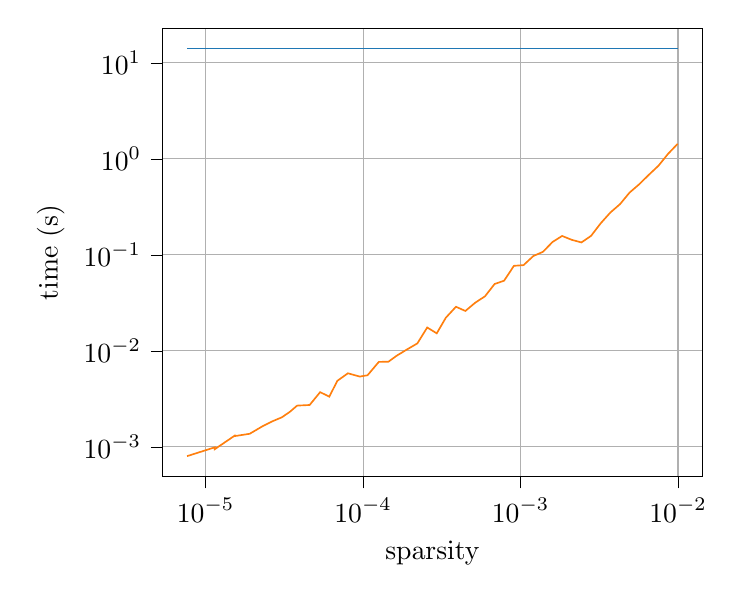
\begin{tikzpicture}

\definecolor{darkgray176}{RGB}{176,176,176}
\definecolor{darkorange25512714}{RGB}{255,127,14}
\definecolor{steelblue31119180}{RGB}{31,119,180}

\begin{axis}[
log basis x={10},
log basis y={10},
tick align=outside,
tick pos=left,
x grid style={darkgray176},
xlabel={sparsity},
xmajorgrids,
xmin=5.32998754456739e-06, xmax=0.014240706792744,
xmode=log,
xtick style={color=black},
xtick={1e-07,1e-06,1e-05,0.0001,0.001,0.01,0.1,1},
xticklabels={
  \(\displaystyle {10^{-7}}\),
  \(\displaystyle {10^{-6}}\),
  \(\displaystyle {10^{-5}}\),
  \(\displaystyle {10^{-4}}\),
  \(\displaystyle {10^{-3}}\),
  \(\displaystyle {10^{-2}}\),
  \(\displaystyle {10^{-1}}\),
  \(\displaystyle {10^{0}}\)
},
y grid style={darkgray176},
ylabel={time (s)},
ymajorgrids,
ymin=0.000491577394963754, ymax=22.9276420956044,
ymode=log,
ytick style={color=black},
ytick={1e-05,0.0001,0.001,0.01,0.1,1,10,100,1000},
yticklabels={
  \(\displaystyle {10^{-5}}\),
  \(\displaystyle {10^{-4}}\),
  \(\displaystyle {10^{-3}}\),
  \(\displaystyle {10^{-2}}\),
  \(\displaystyle {10^{-1}}\),
  \(\displaystyle {10^{0}}\),
  \(\displaystyle {10^{1}}\),
  \(\displaystyle {10^{2}}\),
  \(\displaystyle {10^{3}}\)
}
]
\addplot [semithick, steelblue31119180]
table {%
0.00994873046875 14.0650956392288
0.008636474609375 14.0650956392288
0.00752067565917969 14.0650956392288
0.00652122497558594 14.0650956392288
0.00566291809082031 14.0650956392288
0.00492286682128906 14.0650956392288
0.00428199768066406 14.0650956392288
0.00372314453125 14.0650956392288
0.00323295593261719 14.0650956392288
0.00280570983886719 14.0650956392288
0.00243759155273438 14.0650956392288
0.00211334228515625 14.0650956392288
0.00183677673339844 14.0650956392288
0.00159645080566406 14.0650956392288
0.0013885498046875 14.0650956392288
0.0012054443359375 14.0650956392288
0.00104522705078125 14.0650956392288
0.00090789794921875 14.0650956392288
0.00078582763671875 14.0650956392288
0.000684738159179688 14.0650956392288
0.0005950927734375 14.0650956392288
0.000514984130859375 14.0650956392288
0.000446319580078125 14.0650956392288
0.00038909912109375 14.0650956392288
0.000335693359375 14.0650956392288
0.000293731689453125 14.0650956392288
0.000255584716796875 14.0650956392288
0.00022125244140625 14.0650956392288
0.00019073486328125 14.0650956392288
0.000164031982421875 14.0650956392288
0.00014495849609375 14.0650956392288
0.000125885009765625 14.0650956392288
0.0001068115234375 14.0650956392288
9.5367431640625e-05 14.0650956392288
8.0108642578125e-05 14.0650956392288
6.866455078125e-05 14.0650956392288
6.103515625e-05 14.0650956392288
5.340576171875e-05 14.0650956392288
4.57763671875e-05 14.0650956392288
3.814697265625e-05 14.0650956392288
3.4332275390625e-05 14.0650956392288
3.0517578125e-05 14.0650956392288
2.6702880859375e-05 14.0650956392288
2.288818359375e-05 14.0650956392288
1.9073486328125e-05 14.0650956392288
1.52587890625e-05 14.0650956392288
1.52587890625e-05 14.0650956392288
1.1444091796875e-05 14.0650956392288
1.1444091796875e-05 14.0650956392288
7.62939453125e-06 14.0650956392288
};
\addplot [semithick, darkorange25512714]
table {%
0.00994873046875 1.43381524085999
0.008636474609375 1.12512445449829
0.00752067565917969 0.84903621673584
0.00652122497558594 0.681174516677856
0.00566291809082031 0.542681455612183
0.00492286682128906 0.445064783096313
0.00428199768066406 0.337268114089966
0.00372314453125 0.276551961898804
0.00323295593261719 0.213735818862915
0.00280570983886719 0.157876014709473
0.00243759155273438 0.134737730026245
0.00211334228515625 0.143460273742676
0.00183677673339844 0.157458305358887
0.00159645080566406 0.136191129684448
0.0013885498046875 0.107608079910278
0.0012054443359375 0.0972418785095215
0.00104522705078125 0.0782530307769775
0.00090789794921875 0.0768826007843018
0.00078582763671875 0.0537979602813721
0.000684738159179688 0.049760103225708
0.0005950927734375 0.0370862483978271
0.000514984130859375 0.0317025184631348
0.000446319580078125 0.0260591506958008
0.00038909912109375 0.0288197994232178
0.000335693359375 0.0221850872039795
0.000293731689453125 0.0152351856231689
0.000255584716796875 0.017533540725708
0.00022125244140625 0.0119724273681641
0.00019073486328125 0.0103814601898193
0.000164031982421875 0.00894069671630859
0.00014495849609375 0.00772190093994141
0.000125885009765625 0.00768065452575684
0.0001068115234375 0.00557756423950195
9.5367431640625e-05 0.0054018497467041
8.0108642578125e-05 0.00584697723388672
6.866455078125e-05 0.00487780570983887
6.103515625e-05 0.00333642959594727
5.340576171875e-05 0.00371980667114258
4.57763671875e-05 0.00273275375366211
3.814697265625e-05 0.00269341468811035
3.4332275390625e-05 0.00232267379760742
3.0517578125e-05 0.00203466415405273
2.6702880859375e-05 0.00185537338256836
2.288818359375e-05 0.00163435935974121
1.9073486328125e-05 0.00137090682983398
1.52587890625e-05 0.00129485130310059
1.52587890625e-05 0.00130558013916016
1.1444091796875e-05 0.000947475433349609
1.1444091796875e-05 0.000990629196166992
7.62939453125e-06 0.000801324844360352
};
\end{axis}

\end{tikzpicture}
